\documentclass[10pt,a4paper]{article}
\usepackage[utf8]{inputenc}
\usepackage[italian]{babel}
\usepackage{amsmath}
\usepackage{amsfonts}
\usepackage{amssymb}
\usepackage{graphicx}
\usepackage[left=2cm,right=2cm,top=2cm,bottom=2cm]{geometry}
\newcommand{\rem}[1]{[\emph{#1}]}

\author{Gruppo BN \\ Federico Belliardo, Marco Costa, Lisa Bedini}
\title{Esperienza di Franck-Hertz}
\begin{document}

\maketitle
\section{Scopo dell'esperienza}
Obiettivo dell'esperienza è dimostrare la struttura discreta dei livelli energetici dell'atomo di Neon e di stimarne l'energia di eccitazione mediante lo studio degli effetti dissipativi negli urti anelastici di elettroni su atomi di Neon.\\

\section{Materiale occorrente}
\begin{itemize}
\item Tetrodo a gas Neon ELWE U8482230.
\item Sistema di alimentazione e lettura di corrente ELWE.
\item Oscilloscopio Tektronix TDS 1012.
\end{itemize}

\section{Descrizione esperimento di Franck-Hertz}
L'esperienza prevede lo studio delle collisioni anelastiche elettrone-atomo in un gas di Neon e della relativa fluorescenza indotta dall'eccitazione dei livelli energetici interni. Gli elettroni prodotti per effetto termoionico da un filamento al calor rosso sono accelerati attraverso due griglie di potenziale, tra le quali interagiscono con il Neon, e successivamente raccolti da un anodo dal quale si misura l'intensità di corrente. L'insieme di questi elementi si chiama tetrodo a gas.
Di seguito è riportata la nomenclatura riguardante le tensioni utilizzata nell'esperienza e lo schema circuitale (figura 1):

\begin{itemize}
\item $U_F$: differenza di potenziale applicata al filamento (catodo) rispetto alla terra che ne regola la temperatura, è posta uguale a $U_F = 8.0\pm0.1 \,V$ e tenuta costante.
\item $U_G$: differenza di potenziale applicata alla griglia di controllo rispetto al catodo, regola l'estrazione degli elettroni dal metallo per effetto fotoelettrico a freddo (effetto tunnel). Questa tensione regola l'emissività del catodo, cioè il numero di elettroni emessi per unità di tempo e quindi l'intensità della fluorescenza.
\item $U_A$: differenza di potenziale applicata tra il catodo e la griglia anodo al fine di accelerare gli elettroni, nella configurazione a rampa di potenziale; questo valore indica il massimo potenziale raggiunto dall'anodo.
\item $U_E$: differenza di potenziale tra la griglia anodo e il collettore applicata al fine di stabilire un campo elettrico frenante per gli elettroni che emergono dall'anodo.
\end{itemize}

Un amplificatore operazionale a transimpedenza fornisce in uscita una tensione proporzionale alla corrente di collettore $I_C$.\\

\begin{figure}[!htb]
  \centering
  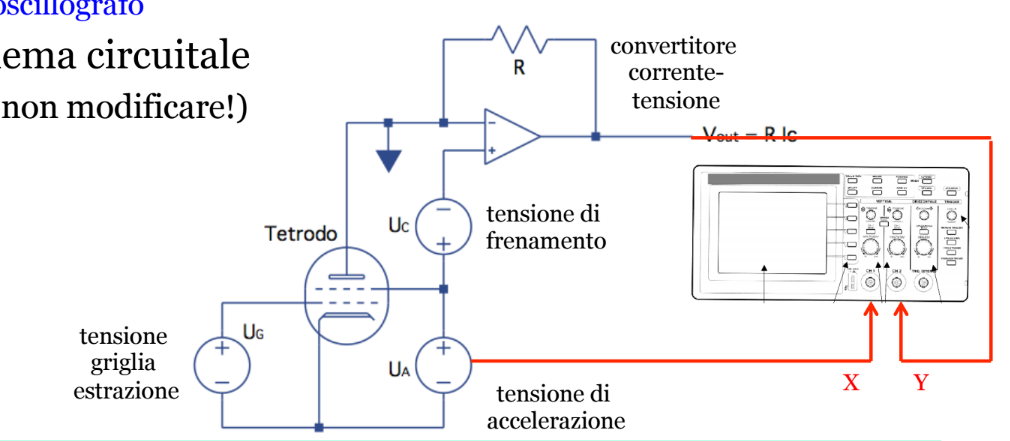
\includegraphics[scale=.5]{circuito.png}
\caption{Schema circuito dell'esperimento e di acquisizione dati.}
\label{circuito}
\end{figure}


\section{Osservazioni qualitative}

Per un valore di $U_G = 3.2 \pm 0.1 \, V $, fisso durante l'esperienza, abbiamo stimato, guardando attraverso la finestra di osservazione, che alle tensioni $U_{A1} = 25 \pm 1 \, V$, $U_{A2} = 41 \pm 1 \, V$, $U_{A3} = 56 \pm 1 \, V$ compaiono in sequenza le barre arancioni. Queste misure sono state ottenute agendo direttamente su $U_A$ in modalità manuale.\\
Per l'errore sulla misura di $U_G$ si è presa l'incertezza strumentale della suddivisione della ghiera con cui si variava la tensione stessa.\\
Il parametro $U_G$ regola la sola intensità della luminescenza (a causa del diverso numero di elettroni che fanno urto elastico) ma non influenza il fatto che la luminescenza appaia o meno.\\
In tutte le operazioni seguenti lavoreremo con il generatore di tensione in modalità rampa e con l'oscilloscopio in modalità XY, dove sull'asse delle ascisse troviamo la tensione $U_A$ e sull'asse delle ordinate la tensione di uscita dell'amplificatore che è proporzionale alla transimpedenza. 
Di seguito sono riportati tre grafici acquisiti con $U_A = 80.0\pm1.0 \, V$ variando la tensione di frenamento $U_E$. L'oscilloscopio è stato posto in modalità XY e abbiamo aumentato la persistenza dell'immagine per una migliore resa dell'immagine.\\


\begin{figure}[!htb]
  \centering
  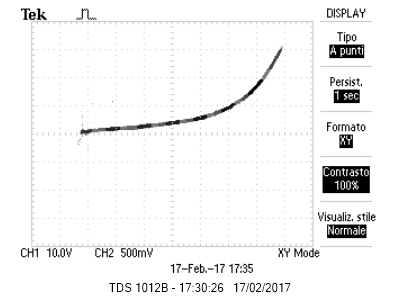
\includegraphics[scale=1.0]{uezero.png}
\caption{Corrente $I_C$ per una tensione $U_E = 0.0\pm0.1 \, V$.}
\label{grafico1}
\end{figure}

\begin{figure}[!htb]
  \centering
  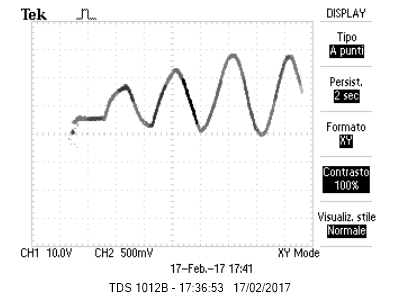
\includegraphics[scale=1.0]{ue9punto680volts.png}
\caption{Corrente $I_C$ per una tensione $U_E = 9.6 \pm 0.1\, V$.}
\label{grafico2}
\end{figure}

%in realtà non è acquisito a 70V...

\begin{figure}[!htb]
  \centering
  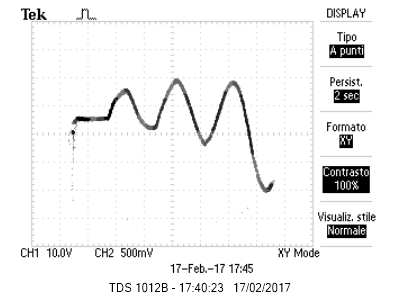
\includegraphics[scale=1.0]{ue10punto970volts.png}
\caption{Corrente $I_C$ per una tensione $U_E = 10.9 \pm 0.1\, V$.}
\label{grafico3}
\end{figure}

%Appunti durante esperienza:
A $U_E = 0.0 \pm0.1\, V$ l'andamento di $I_C$ è monotono in funzione di $U_A$.
Se la differenza di potenziale frenante è nulla non c'è possibilità di frenare gli elettroni e anche quelli che hanno interagito subito prima del ricevente accelerano nel piccolo spazio a disposizione e partecipano alla corrente. Pertanto a $U_E = 0.0\pm0.1\,V$ non si osserva il comportamento oscillante della corrente anche se si vedono le bande luminose.\\ 
Nella fig. \ref{grafico3} si osserva che i minimi della corrente scendono sotto lo zero. Questo significa che per quei valori di tensione la corrente scorre in verso opposto a quello negativo. Non si ritiene che sia un effetto spurio legato all'amplificatore usato ma non si riesce a darne una interpretazione consistente.\\
Variando $U_E$ compaiono i minimi e i massimi e all'aumentare del potenziale di frenamento sono sempre più pronunciati. Per un valore fisso di $U_A$ (massimo potenziale sull'anodo) il numero di minimi e massimi della curva $I_A-U_A$ non cambia al variare di $U_E$.\\

In particolare esiste un valore di $U_E$ per cui i minimi della corrente sono tutti alla stessa altezza, questa situazione come si vede in figura \ref{grafico2} si ottene per $U_E = 9.6 \pm0.1 \, V$.\\

\section{Raccolta ed elaborazione dati}

Di seguito sono riportate le tabelle e i grafici contenti i valori di $U_A$ a cui si osservano i massimi e i minimi della corrente.\\

\begin{table}[!htb]
\centering
\begin{tabular}{|c|c|c|c|}
\hline 
$U_E (V)$ & $U_A (V)$ & $U_A (V)$ & $U_A (V)$ \\ 
\hline 
$2.9\pm0.1\,V$ & $22\pm2$ & $40\pm2$ & $58\pm2$ \\ 
\hline 
$6.0\pm0.1\,V$ & $24\pm2$ & $42\pm2$ & $62\pm2$ \\ 
\hline 
$9.5\pm0.1\,V$ & $28\pm2$ & $46\pm2$ & $66\pm2$ \\ 
\hline 
\end{tabular}
\caption{Tabella dei minimi di $U_A$ in funzione di $U_E$.}
\label{tabellaMinimi} 
\end{table}


\begin{table}[!htb]
\centering
\begin{tabular}{|c|c|c|c|}
\hline 
$U_E (V)$ & $U_A (V)$ & $U_A (V)$ & $U_A (V)$ \\ 
\hline 
$2.9\pm0.1\,V$ & $20\pm2$ & $38\pm2$ & $58\pm2$ \\ 
\hline 
$6.0\pm0.1\,V$ & $18\pm2$ & $35\pm2$ & $55\pm2$ \\ 
\hline 
$9.5\pm0.1\,V$ & $18\pm2$ & $36\pm2$ & $54\pm2$ \\ 
\hline 
\end{tabular} 
\caption{Tabella dei massimi di $U_A$ in funzione di $U_E$.}
\label{tabellaMassimi}
\end{table}

\begin{figure}[!htb]
  \centering
  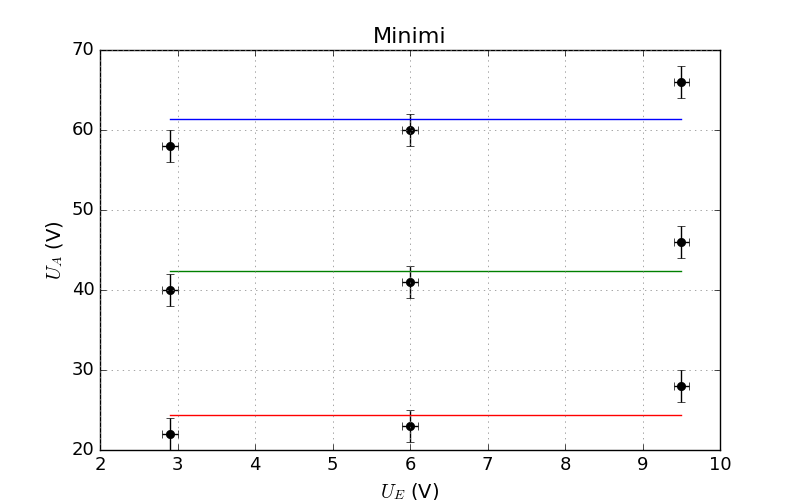
\includegraphics[scale=.7]{min.png}
\caption{Tabella dei minimi di $U_A$ in funzione di $U_E$.}
\label{graficoMin}
\end{figure}

\begin{figure}[!htb]
  \centering
  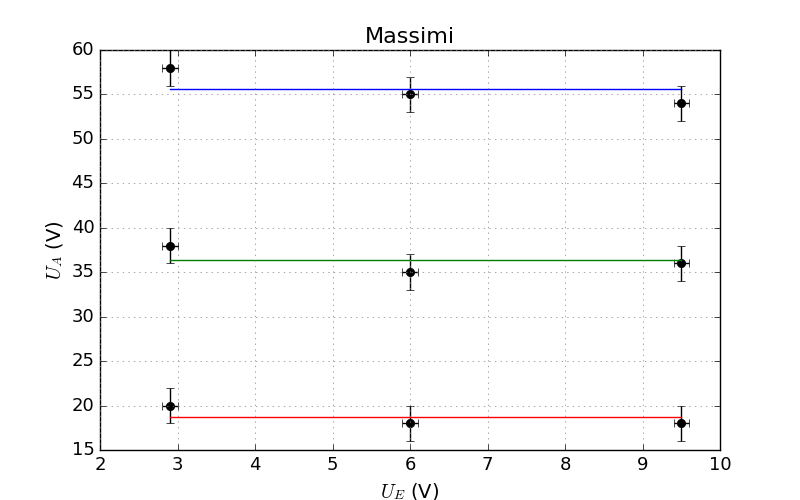
\includegraphics[scale=.7]{max.png}
\caption{Tabella dei massimi di $U_A$ in funzione di $U_E$.}
\label{graficoMax}
\end{figure}

Si sono eseguiti cinque \emph{fit} di costanti utilizzando la funzione \emph{curvefit} della libreria \emph{pylab} con l'opzione \emph{$absolute\,sigma = "true"$}. Di seguito si riportano i valori medi ottenuti dai fit con il relativo errore e $\chi^2$.\\

\begin{table}[!htb]
\centering
\begin{tabular}{|c|c|}
\hline 
$U_A\,(V)$ & $\chi^2 /2$ \\ 
\hline 
$24\pm1$ & $5/2$ \\ 
\hline 
$42\pm1$ & $5/2$ \\ 
\hline 
$61\pm1$ & $8/2$ \\ 
\hline 
\end{tabular}
\caption{Tabella dei minimi medi di $U_A$.}
\label{tabellaMinMed}
\end{figure}

\begin{table}[!htb]
\centering
\begin{tabular}{|c|c|}
\hline 
$U_A\,(V)$ & $\chi^2 /2$ \\ 
\hline 
$18\pm1$ & $0.6/2$ \\ 
\hline 
$36\pm1$ & $1/2$ \\ 
\hline 
$55\pm1$ & $2/2$ \\
\hline
\end{tabular}
\caption{Tabella dei massimi medi di $U_A$.}
\label{tabellaMaxMed}
\end{figure}

I $\chi^2$ associati ai fit delle rete sono migliori nei casi di fit ai massimi che rimangono costanti al variare di $U_E$. Si può vedere che i minimi manifestano in realtà un andamento non banale , si vede infatti che tendono ad aumentare all'aumentare di $U_A$.\\
Di seguito sono riportati i grafici della corrente in unità arbitrarie. Tali grafici sono stati ottenuti dopo un processo di media operato con uno script Python per "ripulire" i dati dagli effetti della digitalizzazione operata dall'acquisizione automatica con l'oscilloscopio.\\
Per ogni dato di tensione $U_A$ l'acquisizione fornisce più dati della corrente. Questo è dovuto al fatto che la rampa viene in realtà salvata sul computer come insieme di gradini a tensione costante e crescenti, a questo \emph{plateau} di tensione viene associato tutto un intervallo di corrente $I_C$ che ovviamente non presenterà \emph{plateau} di digitalizzazione corrispondenti. Ad ogni valore di $U_A$ è associato il punto medio dell'intervallo sopra descritto.

\begin{figure}[!htb]
  \centering
  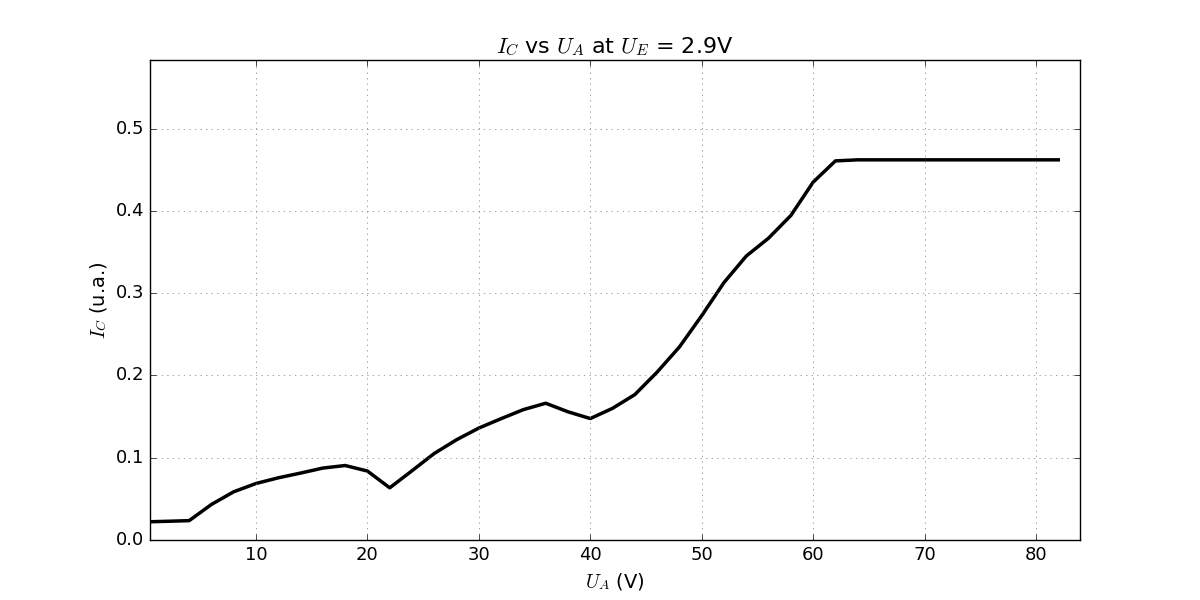
\includegraphics[scale=.5]{plot29.png}
\caption{Grafico della corrente $I_C$ in funzione di $U_A$ a $U_E = 2.9\pm0.1 \, V$.}
\label{grafico4}
\end{figure}

\begin{figure}[!htb]
  \centering
  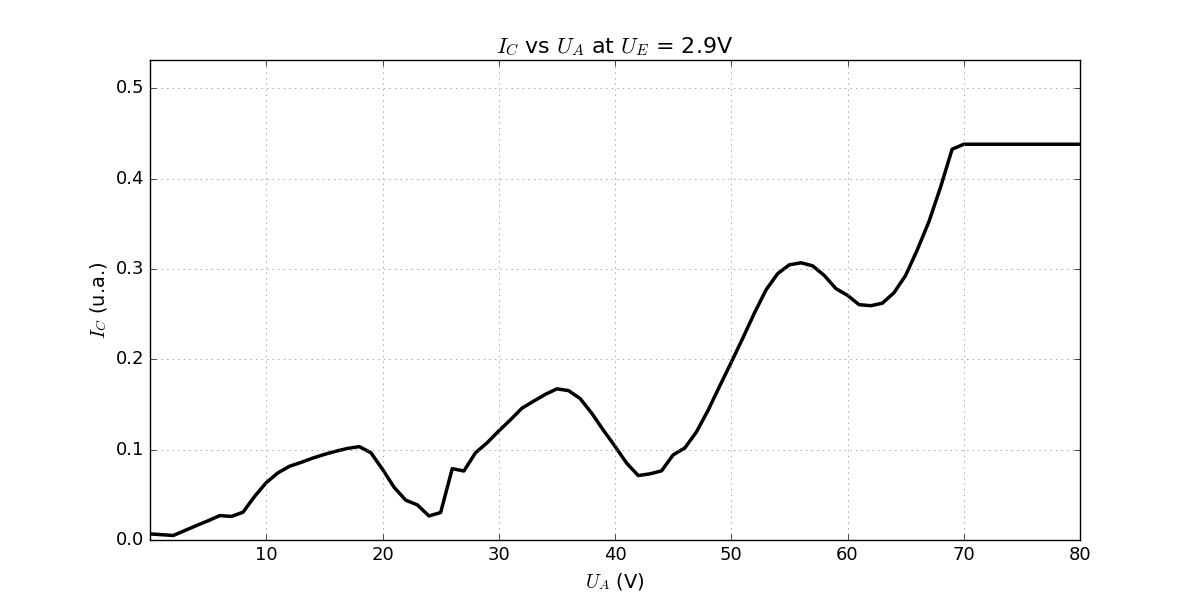
\includegraphics[scale=.5]{plot60.png}
\caption{Grafico della corrente $I_C$ in funzione di $U_A$ a $U_E = 6.0 \pm 0.1\, V$.}
\label{grafico5}
\end{figure}

\begin{figure}[!htb]
  \centering
  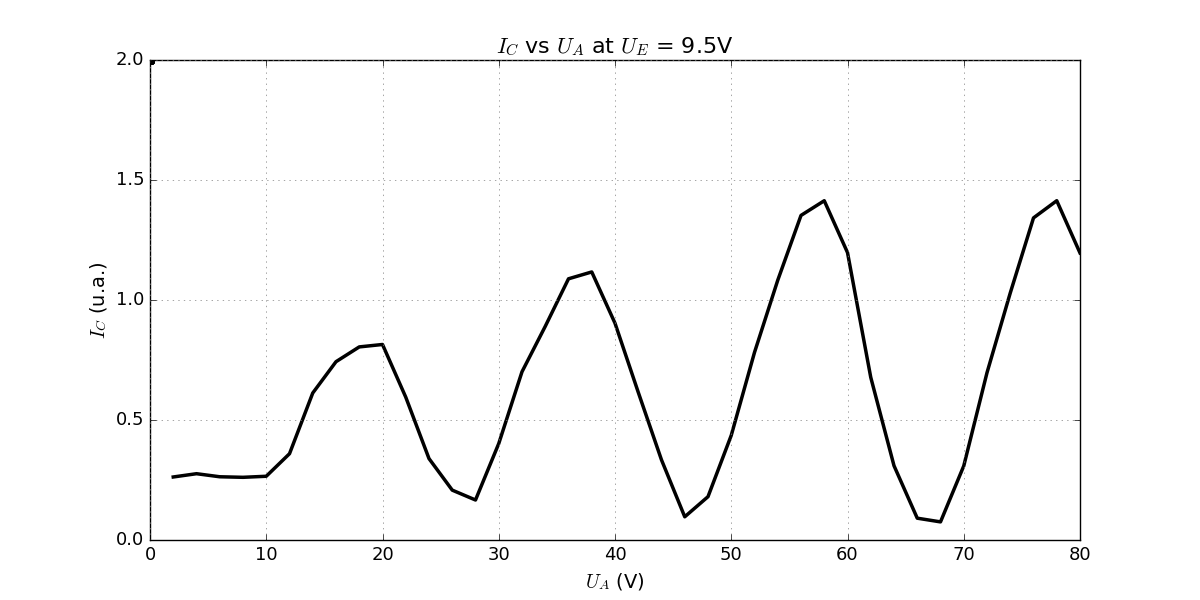
\includegraphics[scale=.5]{plot95.png}
\caption{Grafico della corrente $I_C$ in funzione di $U_A$ a $U_E = 9.5 \pm 0.1\, V$.}
\label{grafico6}
\end{figure}


\section{Conclusioni}
Le tensioni $U_A$ a cui si osservano i massimi sono sistematicamente più basse di quelle misurate al punto 1. Questo può essere dovuto al fatto che il nostro occhio non riusciva a vedere la luminescenza quando ancora troppo flebile, anche se era già cominciato il processo di eccitazione.\\
Il valore di $U_A$ a cui si trovano i minimi aumenta all'aumentare della differenza di potenziale frenante, mentre le posizioni dei massimi rimangono circa costanti.\\
Non si trova un valore di $U_E$ a cui si osservano più nitide le bande di luminescenza.\\
Con i pochi picchi che si sono ottenuti non è pensabile di provare a fornire una stima del cammino libero medio degli elettroni nel Neon. Infatti questo effetto causa una variazione della differenza degli intervalli di potenziale tra i massimi dell'ordine dell'1\% che è dello stesso ordine di grandezza dell'errore, quindi non osservabile.

\end{document}


